\chapter{Knowledge Graphs}
\label{cha:vkg}

\section{Cos'è un Knowledge Graph}
\label{sec:kg_description}

Si inizia a parlare di rappresentazione della conoscenza tramite l'aiuto di knowledge base già dalla fine degli anni 50 e nel 1980 ricercatori dell'università di Groningen 
e dell'università di Twente nei Paesi Bassi usarono per la prima volta il termine Knowledge Graph per descrivere il loro sistema basato sull'integrazione di molteplici sorgenti
di dati per rappresentare il linguaggio naturale tramite una knowledge base .
Questo primo momento di ricerca iniziale fu poi seguito all'inizio degli anni 2000 dall'affermazione degli standard W3C, come RDF e OWL, nell'ambito del 
Semantic Web a dal sorgere di varie ontologie pubbliche come DBPedia, YAGO e Freebase. \cite{KGDefinition} \cite{KGSurvey}

Il termine Knowledge Graph viene però diffuso solo nel 2012 con il motore di ricerca di Google che introduce il termine per descrivere
le nuove funzionalità di ricerca semantica del proprio motore di ricerca: le ricerche che vengono effettuate non sono più semplicemente string matching,
ma viene aggiunta una componente di ragionamento di grado di riconoscere veri e propri "oggetti" del mondo reale. \cite{KGDefinition}

La definizione precisa di cosa sia un Knowledge Graph rimane nebulosa e definizioni differenti risultano essere a volte in contraddizione l'una con l'altra. 
In modo molto generale possiamo definire un Knowledge Graph come una struttura che rappresenta la conoscenza come un insieme di concetti e le relazioni fra essi.
Se vogliamo invece dare una definizione più formale possiamo definire un knowledge graph come una struttura che acquisisce e integra informazioni in una knowledge base
e applica un motore d'inferenza per ricavare nuova conoscenza come mostrato in figura \ref{fig:KG}.
In molte delle definizioni la presenza di una quantità elevata di dati (un ABox di grandi dimensioni) viene spesso considerata un aspetto caratterizzante di un Knowledge Graph,
ma cosa significa nello specifico "qunatità elevata" non è meglio specificato.

La knowledge base è tipicamente implementata tramite un'ontologia, ovvero una struttura a grafo dove i nodi rappresentano gli oggetti e i valori mentre le relazione tra questi 
e le loro proprietà sono rappresentate tramite archi. Questa rappresentazione tramite grafi permette una crescita più flessibile non avendo uno schema definito a priori ed è quindi adatto
per rappresentare domini complessi che attingono dati da fonti molteplici e diversificate tra di loro. Inoltre i linguaggi di interrogazione per strutture a grafo sono molto espressivi e 
contengono la maggior parte dei costrutti usati nei linguaggi di query più tradizionali come join, unioni, proiezioni, \dots \cite{KGIntro}.


\begin{figure}[h]
    \centering
    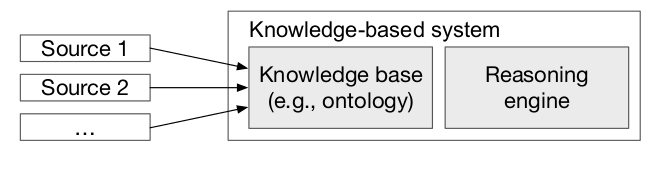
\includegraphics[width = 0.75\linewidth]{KG}
    \caption{Struttura di un KG}
    \label{fig:KG}
\end{figure}


\section{Virtual Knowledge Graph}
\label{sec:vkg_description}
I virtual knowledge graph applicano al concetto di knowledge graph quello di data virtualization. Questo significa che l'ontologia in un VKG l'ontologia non viene materializzata, ma viene dichiarato un insieme di mapping 
che permette di tradurre un insieme di concetti e proprietà tipiche di un'ontologia in un query SQL che vengono eseguite direttamente sulle sorgenti relazionali. 

Da un punto di vista più formale possiamo considerare la specifica di un Virtual Knowledge Graph come una tupla P = (O, M, S) dove abbiamo:
\begin{itemize}
    \item ontologia O: rappresentazione a grafo del dominio in analisi con un vocabolario rappresentativo del dominio. 
        In questo modo viene implementata una separazione tra i dettagli di basso livello delle fonti e la visione d'insieme data dall'ontologia che permette così anche a persone esperte nel campo, ma nell'integrazione 
        dei dati di ricavare informazioni. 
        In particolare W3C presenta vari standard per la rappresentazione delle ontologie tra cui i principali RDFS e OWL, entrambi basati sullo standard RDF (Resource Description Network) usato per descrivere grafi e al 
        fine di interrogare questo grafo lo standard è SPARQL.
    \item mapping M: insieme di affermazioni che specifica come le classi e le proprietà presenti nell'ontologia siano popolate da dati provenienti dalle sorgenti. Formalmente, dato lo schema di un database S e 
        un'ontologia O, un'affermazione di mapping tra S e O è un espressione in una di queste forme:
        \[ \phi(x) \leadsto (f(x) \ \textrm{rdf:type A}) \]
        \[\phi(x, x') \leadsto (f(x) \ P \ f'(x'))\] 
        dove $f$ è un costruttore di termini RDF ovvero una funzione che mappa una tupla di un database a una URI o un letterale RFD.
        In altre parole tutte le tuple del database vengono tradotte dando informazioni o sul tipo di dato o su relazioni di tipo (soggetto, predicato, oggetto)
        Lo standard per i mapping tra RDF e database relazionali fornito da W3C è R2RML.
    \item schema S: struttura delle sorgenti dati, tipicamente database relazionali.
\end{itemize}

A questo punto possiamo definire un'istanza di un Virtual Knowledge Graph come la coppia (P, D) dove P = (O, M, S) è la specifica di un VKG istanziata su un database D che rispetta lo schema S.
Dati M e D le triple generate applicando M su D costituiscono il grafo RDF che definisce il significato semantico dell'intero sistema.

Se vogliamo caratterizzare un Virtual Knowledge Graph sotto il punto di vista della logica descrittiva allora possiamo considerare l'ontologia come un TBox e le informazioni ricavate dalle sorgenti 
tramite i mapping come l'ABox \cite{OBDA} \cite{VKGOverview}. 


\begin{figure}[h]
    \centering
    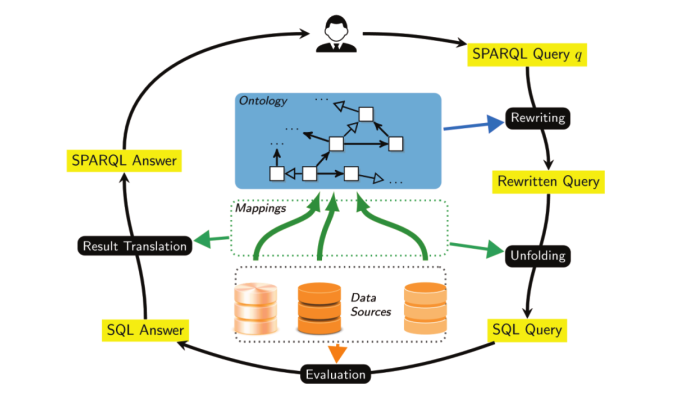
\includegraphics[width = 0.75\linewidth]{VKGRewriting.png}
    \caption{Riscrittura di una query in un VGK}
    \label{fig:VKGRewriting}
\end{figure}


\section{Il Virtual Knowledge Graph system Ontop}
\label{sec:vkg_ontop}

Ontop è un Virtual Knowledge Graph system open-source sviluppato dalla Libera Università di Bolzano e dall'azienda Ontopic s.r.l. . Riceve inoltre
contributi importanti da Birkbeck, University of London.

Ontop supporta glli standard W3C in materia di ontologie e Knowledge Graph; in particolare supporta RDF 1.1 come modello per i grafi, RDFS e OWL 2 QL per le
ontologie, R2RML e un sistema di mapping di Ontop che può essere tradotto in R2RML per i mapping e supporta la maggior parte dei costrutti presenti in SPARQL 1.1.
Inoltre, nonostante sia un VKG permette di materializzare il grafo RDF se necessario. \cite{OntopSite}

\subsection{Intermediate Query language}
Ontop era inizialmente basato su Datalog poi passato ad un proprio linguaggio interno (Intermediate Query)

IQ: rappresentazione usata per tradurre le query degli utenti in SPARQL nelle query SQL dei mapping

\subsection{Esempi di utilizzo}
Esempi di utilizzo di Ontop in ambienti aziendali e accademici


